%==============================================================
%  Appendix A -- Code & Supplementary Material
%  (does not count towards the 4-page limit, per the CO3 brief)
%==============================================================
\chapter{Supplementary Material}
\label{app:supp}

%--------------------------------------------------------------
\section{Lagrange--Newton implementation}
\label{app:code}
%--------------------------------------------------------------

Listing~\ref{lst:ln} reproduces the complete driver used to
produce the Lagrange--Newton results in
Section~\ref{sec:results}. The parameter vectors, objective,
gradient, constraint and solver call correspond one-to-one with
the formulation in Section~\ref{sec:formulation}. Both listings
are also available in the project repository:
\url{https://github.com/the-nerd-sloth/co3-semester-project.git}

\vspace{0.5cm}
{\captionsetup{justification=raggedright,singlelinecheck=false}
\lstinputlisting[
    style=pythonstyle,
    language=Python,
    caption={Lagrange--Newton baseline (\texttt{Code/lagrange\_newton.py}). Runs in $<1$~s on a standard laptop and reproduces the numbers quoted in Section~\ref{sec:results}.},
    label={lst:ln}
]{Code/lagrange_newton.py}}

%--------------------------------------------------------------
\section{Simulated Annealing implementation}
\label{app:sa}
%--------------------------------------------------------------

Listing~\ref{lst:sa} gives the self-contained SA driver.
The key design decisions are (i)~the feasibility-preserving
pairwise transfer move of equations~\eqref{eq:coupled}--\eqref{eq:deltamax},
which avoids \texttt{np.clip} after the perturbation step and
thereby keeps $\sum_i a_i x_i = S$ exact throughout; and
(ii)~the linear cooling schedule~\eqref{eq:cooling} with
$T_0 = 500$ and $k_{\max}=50{,}000$ as specified in CO3 Chapter~7.

\vspace{0.5cm}
{\captionsetup{justification=raggedright,singlelinecheck=false}

\lstinputlisting[
    style=pythonstyle,
    language=Python,
    caption={Simulated Annealing implementation (\texttt{Code/simulated\_annealing.py}).
    The constraint-preserving transfer move ensures strict feasibility at every step
    without any projection or rejection.},
    label={lst:sa}
]{Code/simulated_annealing.py}}

%--------------------------------------------------------------
% Supplementary tables and figures (no section headings --
% presented as self-contained floats with captions)
%--------------------------------------------------------------


\begin{table}[h]
\centering
\small
\caption{SA robustness across five independent random seeds
($S=3500$~L/day, $T_0=500$, $k_{\max}=50{,}000$, \texttt{step\_size}$=20$).
The gap $\delta f = f_{\text{SA}}^* - f_{\text{LN}}^*$ measures how far
each run is from the Lagrange--Newton reference $f_{\text{LN}}^* = 133{,}446$.
The maximum relative gap of $0.036\,\%$ confirms SA robustness to initialisation.}
\label{tab:robustness}
\begin{tabular}{@{}crrr@{}}
\toprule
Seed & $f_{\text{SA}}^*$ & $\delta f$ (L$^2$/day$^2$) & Relative gap (\%) \\ \midrule
 0  & 133\,466 & 20  & 0.015 \\
 1  & 133\,485 & 40  & 0.030 \\
 2  & 133\,494 & 48  & 0.036 \\
 3  & 133\,483 & 37  & 0.028 \\
42  & 133\,475 & 30  & 0.022 \\
\midrule
Mean & 133\,481 & 35 & 0.026 \\
\bottomrule
\end{tabular}
\end{table}

\begin{table}[h]
\centering
\small
\caption{Full 20-row allocation table for the base scenario ($S=3500$~L/day).
The vectors $\mathbf{a}$ and $\mathbf{w}$ are linearly spaced:
$a_i = 1.00 + 0.25\,(i-1)/(n-1)$ and $w_i = 1.00 + 0.80\,(i-1)/(n-1)$,
so that household~1 is the easiest to serve and least prioritised
while household~20 is the most pipe-lossy and most vulnerable.
Both methods produce the interior water-filling solution~\eqref{eq:waterfilling}
throughout; no box bound is active.}
\label{tab:full_alloc}
\begin{tabular}{@{}ccccrr@{}}
\toprule
$i$ & $a_i$ & $w_i$ & $d_i$ (L/day) & $x^*_{\text{LN}}$ (L/day) & $x^*_{\text{SA}}$ (L/day) \\ \midrule
 1 & 1.000 & 1.000 & 225 & 148.01 & 144.86 \\
 2 & 1.013 & 1.042 & 225 & 149.22 & 146.30 \\
 3 & 1.026 & 1.084 & 225 & 150.31 & 147.75 \\
 4 & 1.039 & 1.126 & 225 & 151.29 & 149.01 \\
 5 & 1.053 & 1.168 & 225 & 152.18 & 150.23 \\
 6 & 1.066 & 1.211 & 225 & 152.99 & 151.49 \\
 7 & 1.079 & 1.253 & 225 & 153.73 & 152.55 \\
 8 & 1.092 & 1.295 & 225 & 154.41 & 153.44 \\
 9 & 1.105 & 1.337 & 225 & 155.04 & 154.37 \\
10 & 1.118 & 1.379 & 225 & 155.62 & 155.30 \\
11 & 1.132 & 1.421 & 225 & 156.16 & 156.04 \\
12 & 1.145 & 1.463 & 225 & 156.67 & 156.84 \\
13 & 1.158 & 1.505 & 225 & 157.14 & 157.56 \\
14 & 1.171 & 1.547 & 225 & 157.58 & 158.21 \\
15 & 1.184 & 1.589 & 225 & 157.99 & 158.83 \\
16 & 1.197 & 1.632 & 225 & 158.38 & 159.53 \\
17 & 1.211 & 1.674 & 225 & 158.75 & 160.05 \\
18 & 1.224 & 1.716 & 225 & 159.10 & 160.67 \\
19 & 1.237 & 1.758 & 225 & 159.43 & 161.18 \\
20 & 1.250 & 1.800 & 225 & 159.74 & 161.77 \\
\bottomrule
\end{tabular}
\end{table}

\begin{figure}[h]
\centering
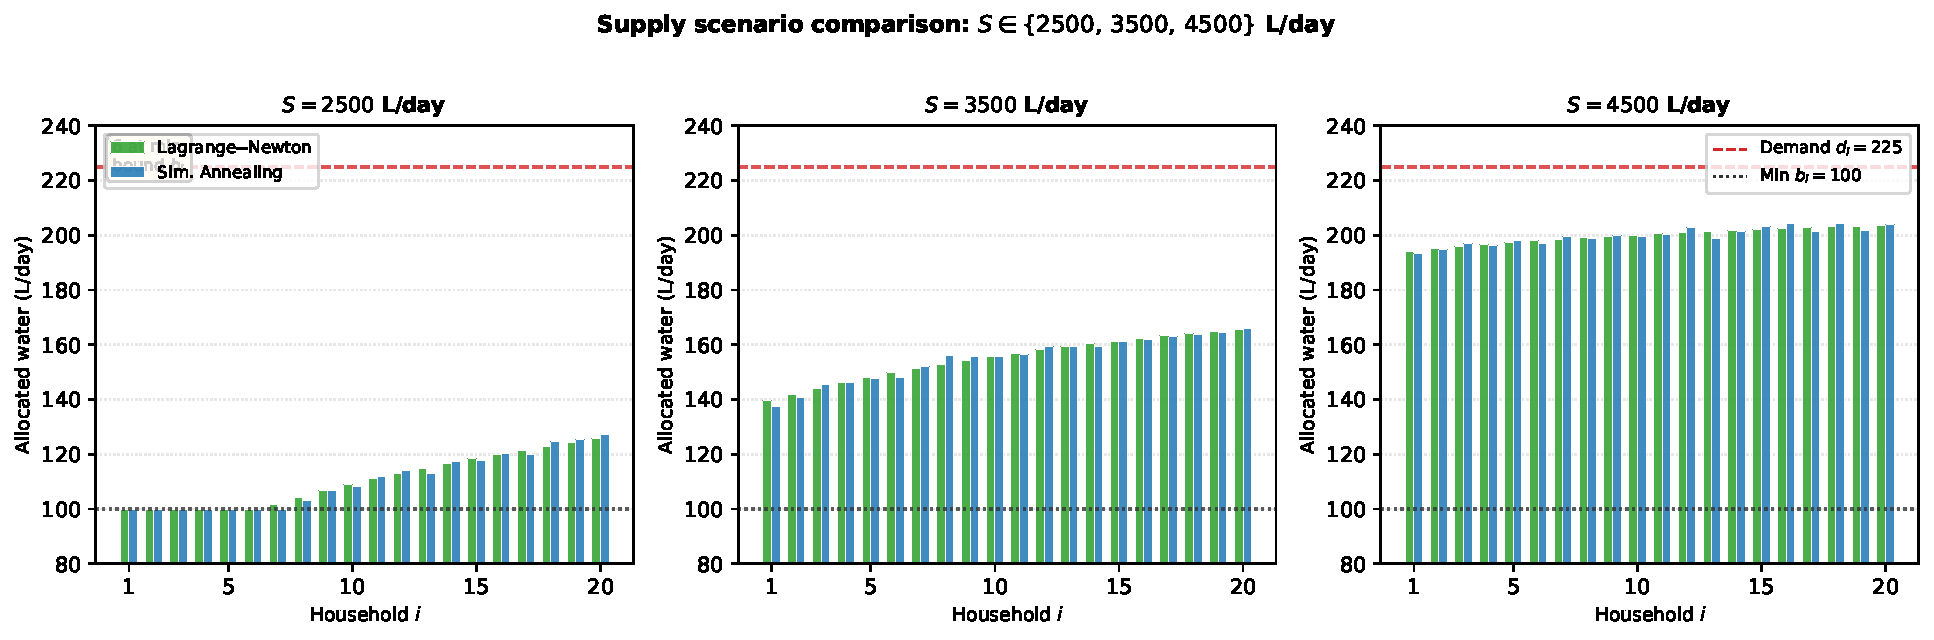
\includegraphics[width=\linewidth]{Figures/fig_scenarios.pdf}
\caption{Supply scenario comparison for $S \in \{2500,\,3500,\,4500\}$~L/day.
At $S=2500$~L/day (left panel) the lower box bound $b_i = 100$~L/day becomes
active for the six most pipe-lossy households ($a_i \geq 1.17$), confirming
the feasibility boundary analysis in Section~\ref{sec:formulation}.
At $S=3500$~L/day (centre) all households are interior and the water-filling
solution~\eqref{eq:waterfilling} applies throughout.
At $S=4500$~L/day (right) supply exceeds demand for the least pipe-lossy
households, but capping at $d_i=225$~L/day prevents over-delivery.
Both methods track each other closely across all three scenarios.}
\label{fig:scenarios}
\end{figure}

\begin{figure}[h]
\centering
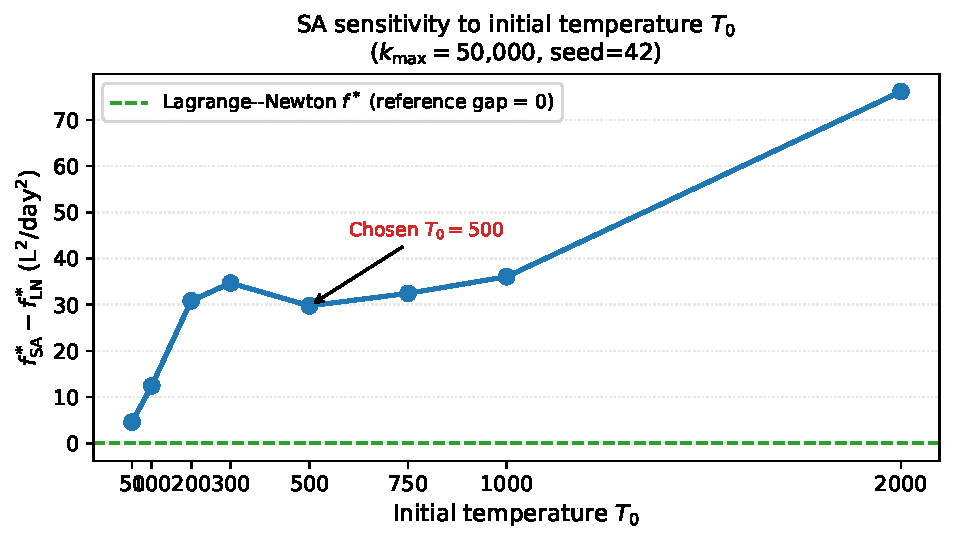
\includegraphics[width=0.72\linewidth]{Figures/fig_T0_sensitivity.pdf}
\caption{SA final objective gap $f_{\text{SA}}^* - f_{\text{LN}}^*$ as a
function of initial temperature $T_0$ ($k_{\max}=50{,}000$, \texttt{seed=42}).
The gap remains below $40$~L$^2$/day$^2$ across the full range tested,
confirming low sensitivity to $T_0$.  The chosen value $T_0=500$ (arrow)
balances early exploration with adequate final exploitation; very low $T_0$
($\leq 100$) reduces exploration and marginally increases the gap.}
\label{fig:T0}
\end{figure}
